Before we begin defining our problem, we need to introduce a small amount of notation.

\subsection{Vectors}

\begin{description}
  \item[$\bvec{a}$] Vector in n-dimensional space.
  \item[$\bhat{a}$] Unit vector in n-dimensional space. $\bhat{a} = \bvec{a}/a$ and $\norm{\bhat{a}} = 1$.
  \item[$a$] Scalar quantity. Usually $a = \norm{\bvec{a}}$, but occasionally we will also define a sign that is dependent on the direction of $\bhat{a}$.
\end{description}

\subsection{Angles}

We define a directional angle measurement, which we will use throughout the paper. All angles are in $[-\pi, \pi]$, and the positive measurement direction is indicated by an arrow on the angle.

\begin{figure}[H]
  \begin{subfigure}[b]{0.3\textwidth}
    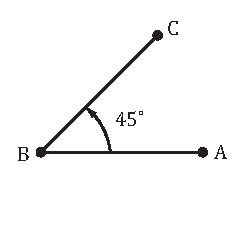
\includegraphics[width=\textwidth]{angle_def_3.eps}
    \caption{}
    \label{fig:angle-def-3}
  \end{subfigure}
  \qquad \qquad
  \begin{subfigure}[b]{0.3\textwidth}
    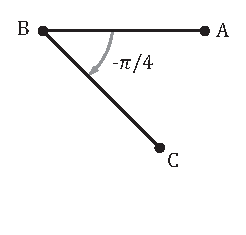
\includegraphics[width=\textwidth]{angle_def_4.eps}
    \caption{}
    \label{fig:angle-def-4}
  \end{subfigure}
  \caption{Directional angle notation}
\end{figure}
